% $Id$

%==============================================================================
\chapter{Component Programming Model}
%==============================================================================

%------------------------------------------------------------------------------
\section{Overview}
%------------------------------------------------------------------------------

After writing our first component, we are ready to learn more about the 
component programming model.
When we are talking about component based development, we have to realize that there 
are two different views on the same component:
\begin{itemize}
\item {\bf Client's view}: As shown in the last section, a client finds a component 
home, creates a component instance and uses operations provided by the component's facets.

\item {\bf Business logic's view}: To implement some business logic, the component
developer has to know the programming API of the used component model.
There is a contract between the written code and the component's runtime environment.
The component container provides a {\it context object} that allows the component
instance to get information about its environment. In the other direction, the
component implements {\it callback methods} that are called by the container if any
life--cycle event occurs.
\end{itemize}

\begin{figure}[htbp]
    \begin{center}
        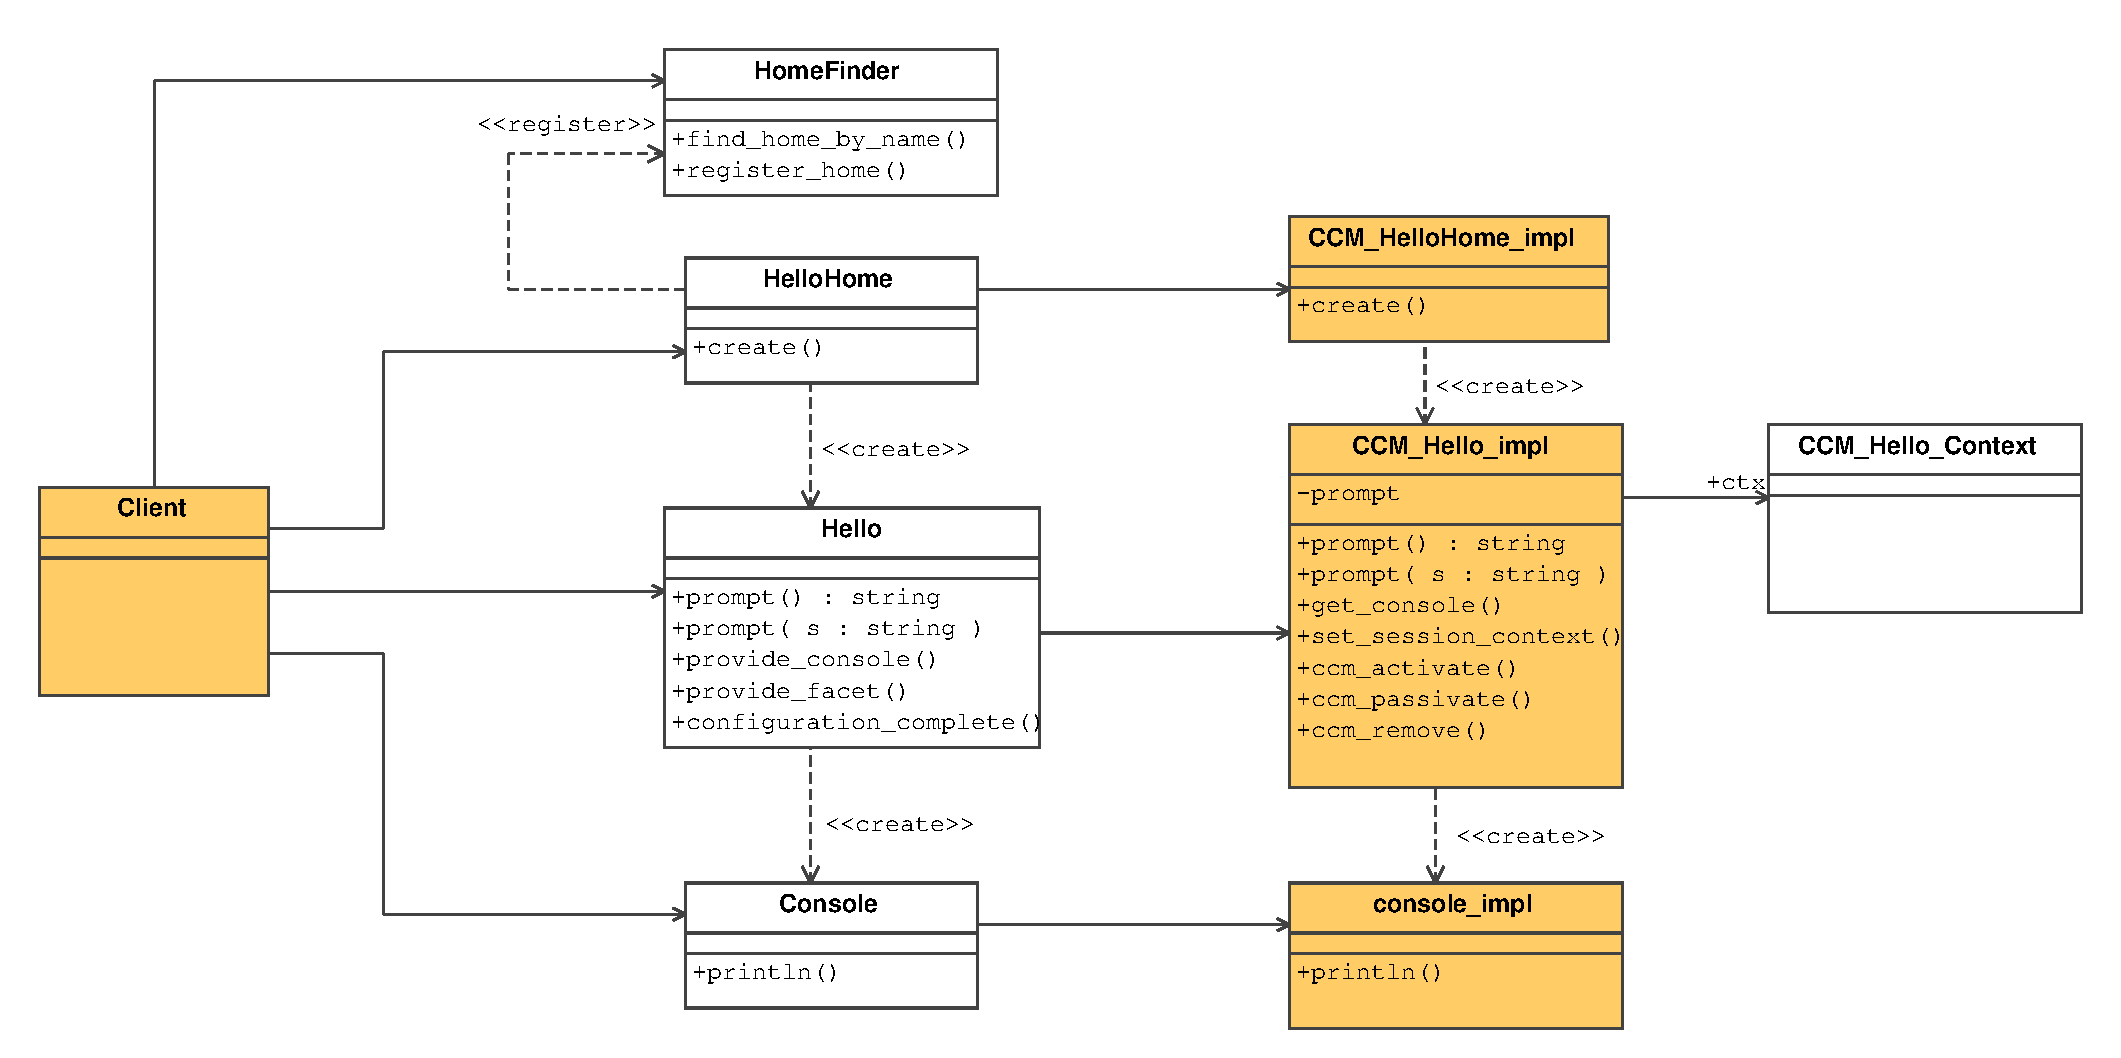
\includegraphics [width=12cm,angle=0] {ComponentViews.eps}
        \caption{Client side and business logic view on the same component}
        \label{fig:ComponentViews}
    \end{center}
\end{figure}


%------------------------------------------------------------------------------
\section{Client's View}
%------------------------------------------------------------------------------

The client interacts with generated classes that are part of the component's
runtime environment. These adapter classes are generated from the definitions
in the IDL3 file.
Keep in mind, that a client never calls methods on the component's implementation
classes directly, every client call is intercepted by the component container. 

\begin{figure}[htbp]
    \begin{center}
        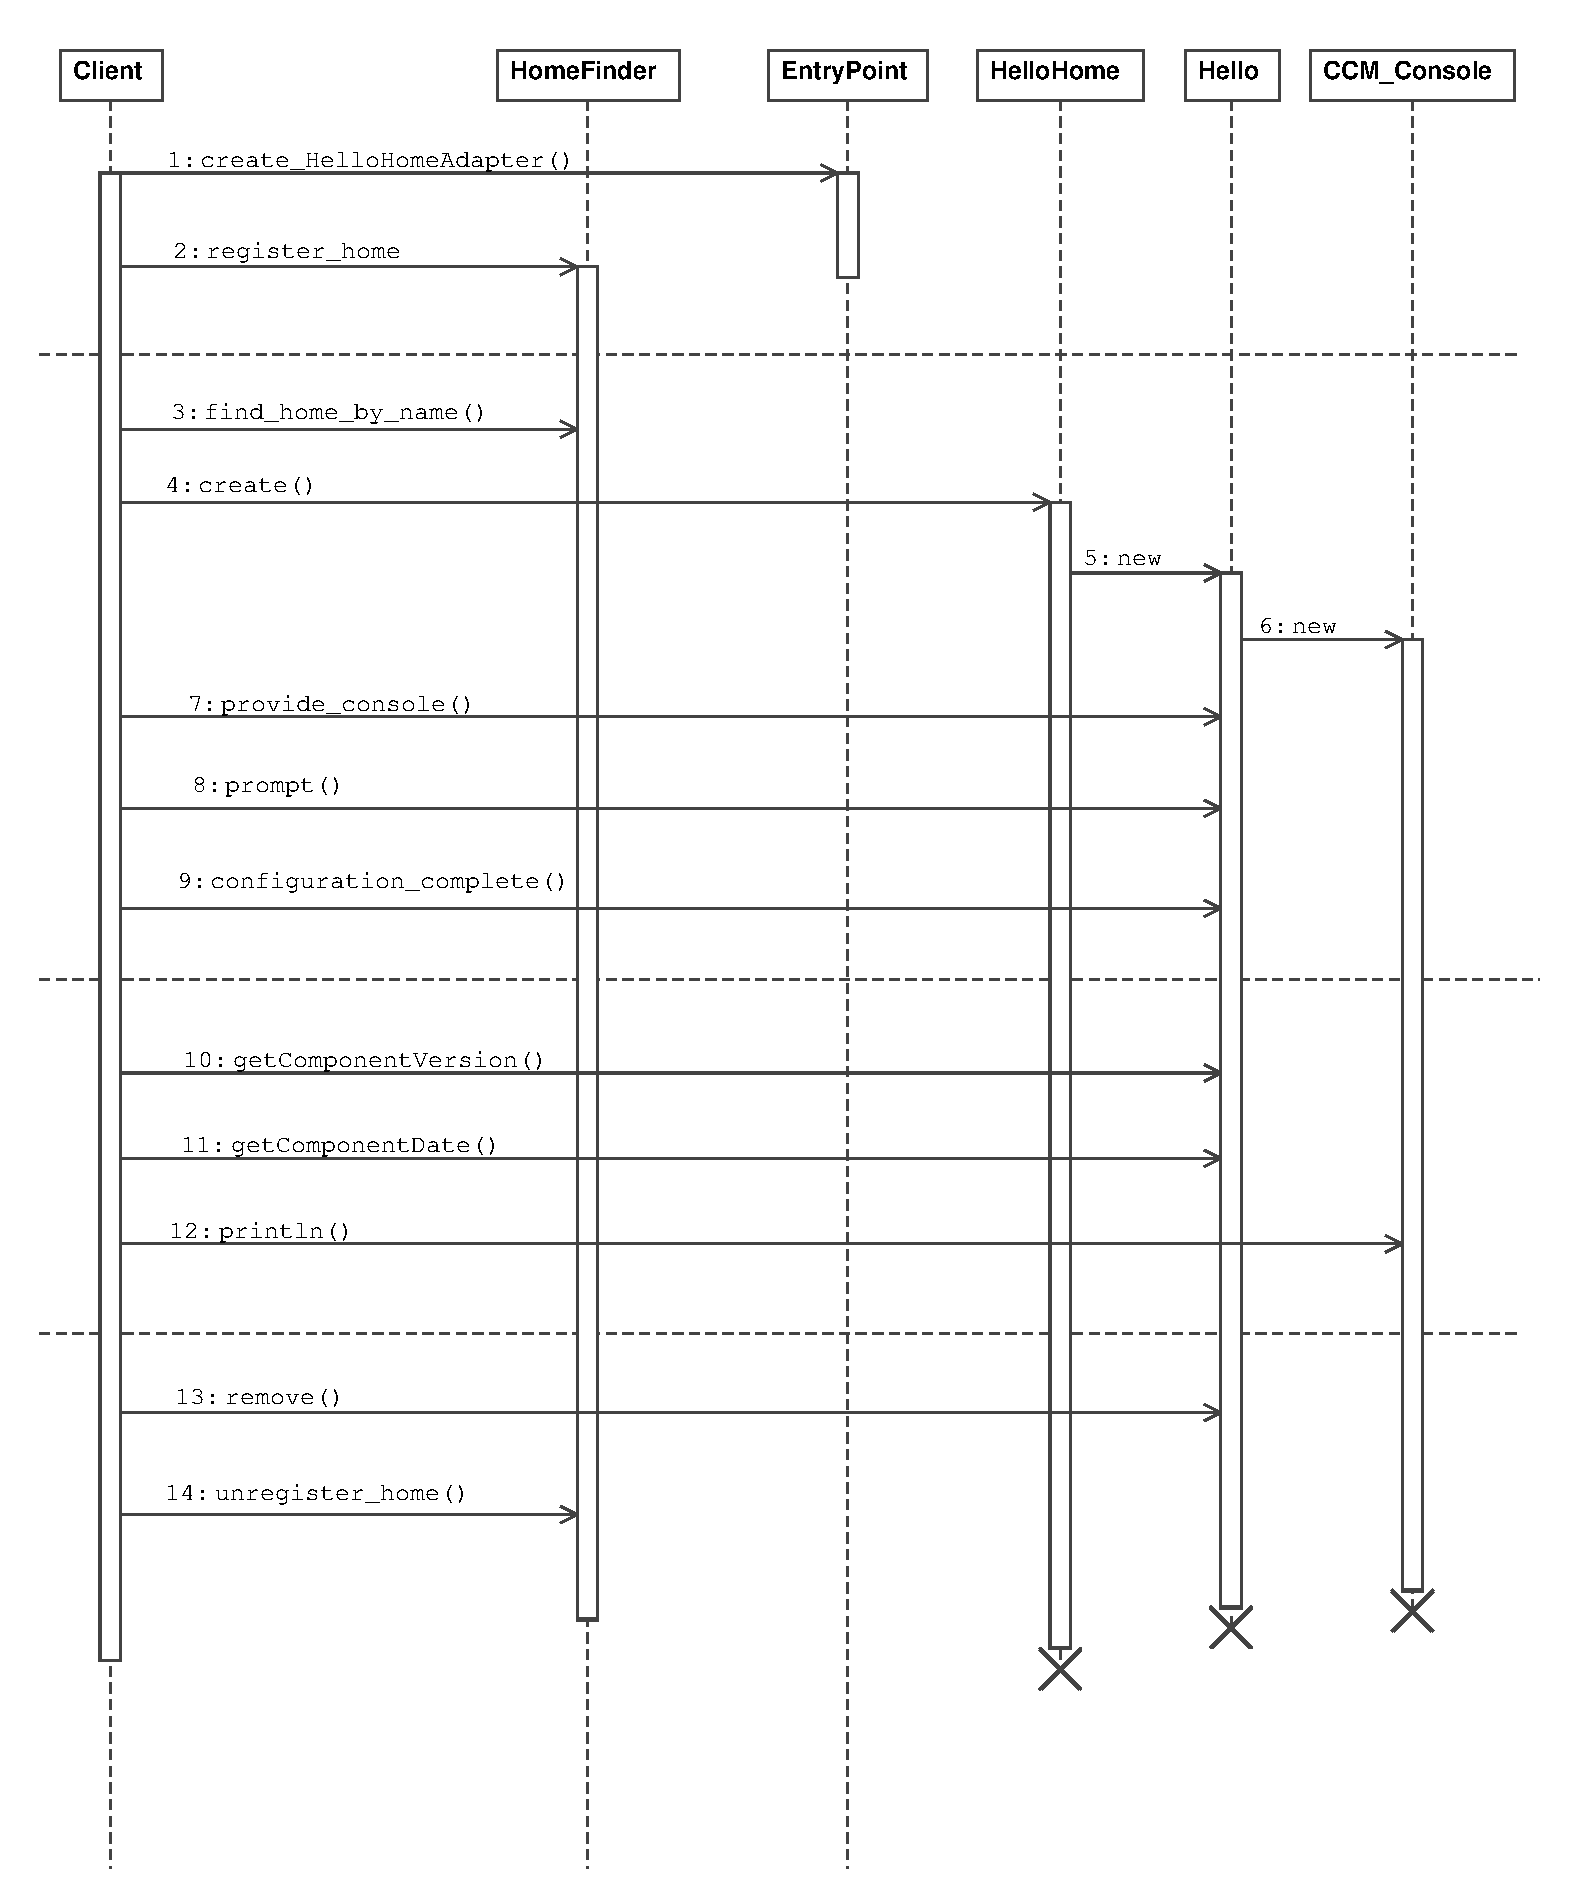
\includegraphics [height=16cm,angle=0] {ClientView.eps}
        \caption{Client to component interaction}
        \label{ClientView}
    \end{center}
\end{figure}

\noindent
The related client code has been shown in the last chapter.
Note that the adapter classes are referenced via smart pointers. Therefore,
the adapters are deleted after their references go out of scope.


%------------------------------------------------------------------------------
\section{Business Logic's View}
%------------------------------------------------------------------------------

The component implementation only interacts with the component environment.
Each client call is delegated through the container to the implementation class.
The component's life--cycle is controlled by the container using callback methods.

\begin{figure}[htbp]
    \begin{center}
        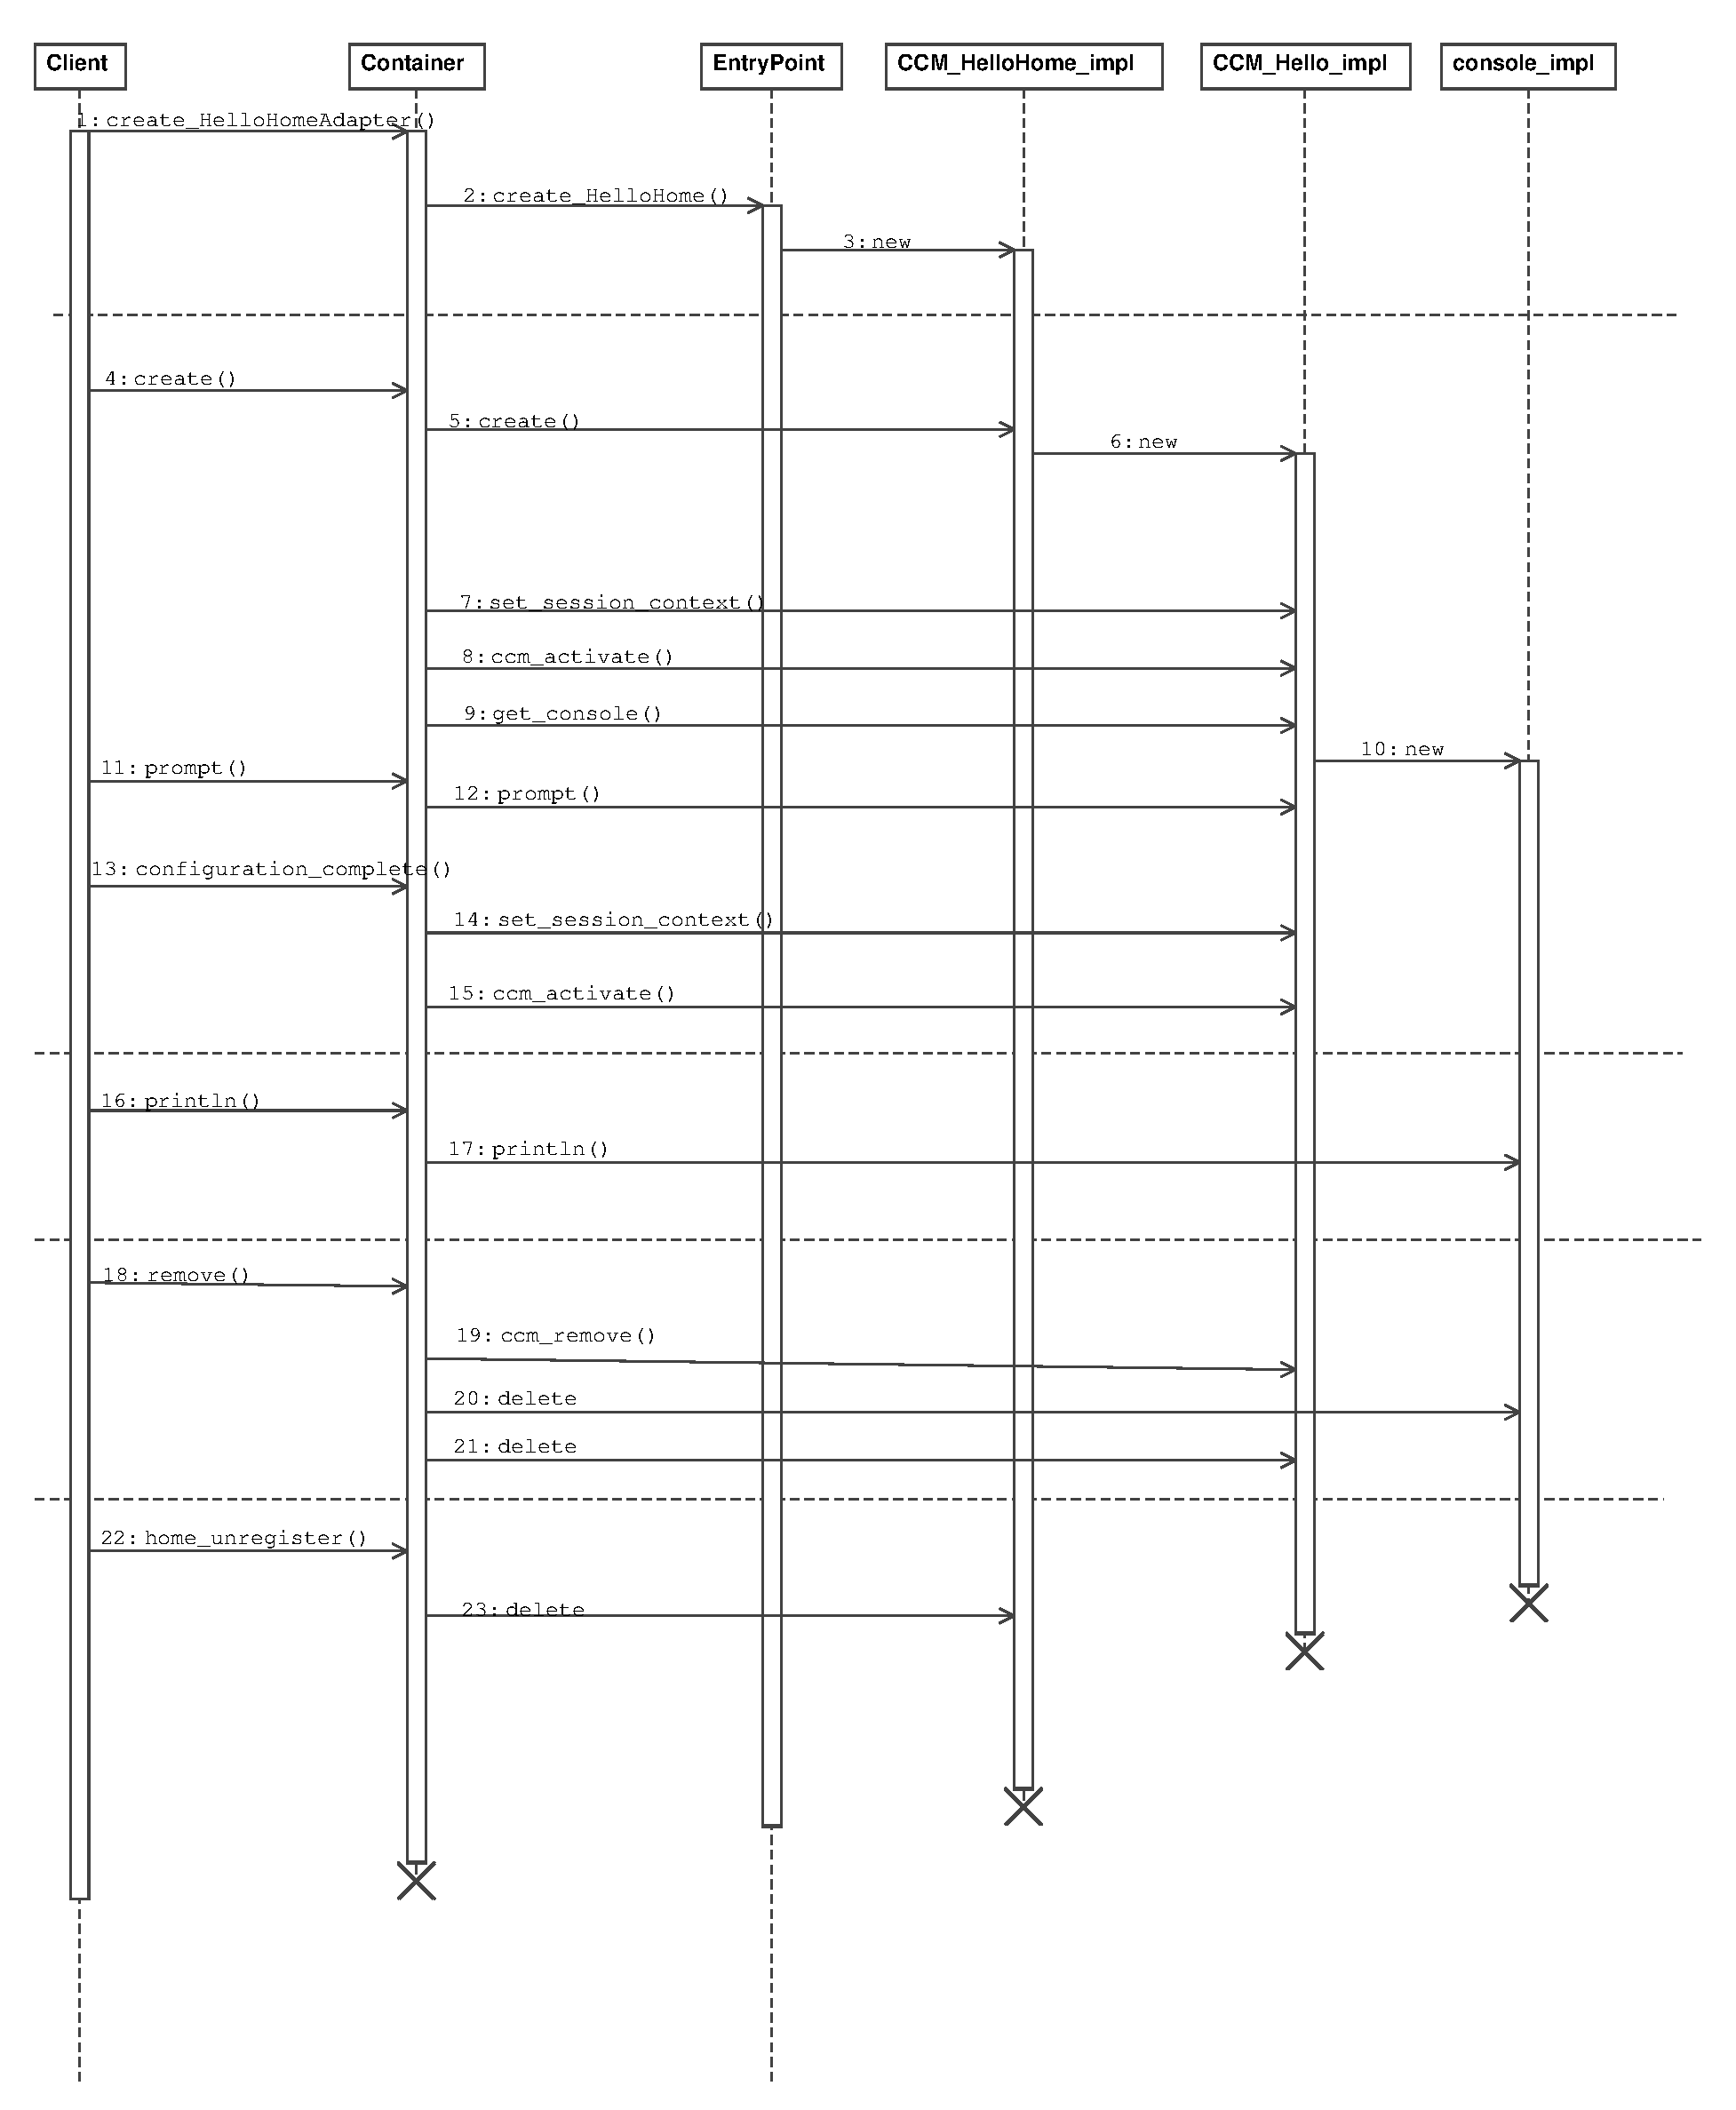
\includegraphics [height=17cm,angle=0] {BusinessLogicView.eps}
        \caption{Container and component interaction}
        \label{BusinessLogicView}
    \end{center}
\end{figure}


With the following source code, we describe the classes that must be written to 
implement a component, as shown in figure \ref{fig:ComponentViews}.
Remember, the component developer only has to consider the contract between the
component and its container.

After writing the IDL3 file, we can hack the code that realizes the component's
home:
\begin{small}
\begin{verbatim}
/**
 * HelloHome_app.h file
 **/

#ifndef __HelloHome__APP__H__
#define __HelloHome__APP__H__
#include "HelloHome_gen.h"

namespace CCM_Local {
namespace CCM_Session_Hello {

class CCM_HelloHome_impl
  : public CCM_HelloHome
{
 public:
  virtual localComponents::EnterpriseComponent* create()
    throw (localComponents::CCMException);
};

} // /namespace CCM_Session_Hello
} // /namespace CCM_Local

extern "C" {
  localComponents::HomeExecutorBase* create_HelloHome();
}

#endif
\end{verbatim}
\end{small}

\begin{small}
\begin{verbatim}
/**
 * HelloHome_app.cc file
 **/

#include "HelloHome_app.h"

using namespace std; 
namespace CCM_Local {
namespace CCM_Session_Hello {

/**
 * The create() method instantiates a new component class and returns the
 * pointer to the container.
 * Note that the result is of type localComponents::EnterpriseComponent*
 * The container is responsible to delete the component class instance. 
 **/
localComponents::EnterpriseComponent* CCM_HelloHome_impl::create()
  throw (localComponents::CCMException)
{
  return dynamic_cast<localComponents::EnterpriseComponent*> (new CCM_Hello_impl());
}

} // /namespace CCM_Session_Hello
} // /namespace CCM_Local

/**
 * This is the entry point for the business logic. The container calls this
 * factory method to get a pointer to the home class implementation.
 * Note that the return value is of type localComponents::HomeExecutorBase*
 * The container is responsible to delete the home class instance.
 **/
extern "C" {
  localComponents::HomeExecutorBase* create_HelloHome()
  {
    return new CCM_Local::CCM_Session_Hello::CCM_HelloHome_impl();
  }
}
\end{verbatim}
\end{small}

\noindent
While the component home creates the instances of a component type, the component's 
business logic is coded within the component and the facet classes:

\begin{small}
\begin{verbatim}
/**
 * Hello_app.h file
 **/

#ifndef __Hello__APP__H__
#define __Hello__APP__H__

#include "Hello_gen.h"

namespace CCM_Local {
namespace CCM_Session_Hello {

class CCM_Hello_impl
  : public CCM_Hello
{
 private:
  std::string prompt_;

 public:
  CCM_Hello_Context* ctx;

  std::string prompt();
  void prompt(std::string value);

  CCM_Console* get_console();

  void set_session_context (localComponents::SessionContext* ctx)
    throw (localComponents::CCMException);
  void ccm_activate()
    throw (localComponents::CCMException);
  void ccm_passivate()
    throw (localComponents::CCMException);
  void ccm_remove()
    throw (localComponents::CCMException);
};


class console_impl
  : public CCM_Console
{
 private:
  CCM_Hello_impl* component;

 public:
  console_impl(CCM_Hello_impl* component_impl);
  long println(const std::string& s);
};

} // /namespace CCM_Session_Hello
} // /namespace CCM_Local

#endif
\end{verbatim}
\end{small}


\begin{small}
\begin{verbatim}
/**
 * Hello_app.cc file
 **/

#include <iostream>
#include "Hello_app.h"

using namespace std;
using namespace CCM_Utils;

namespace CCM_Local {
namespace CCM_Session_Hello {

/**
 * This method instantiates a facet class and returns the instance pointer
 * of type CCM_Console* to the container.
 * The container is responsible to delete the facet class instance.
 * Note that the name of the get_*() method corresponds with the facet name.
 **/
CCM_Console* CCM_Hello_impl::get_console()
{
  console_impl* facet = new console_impl(this);
  return dynamic_cast<CCM_Console*>(facet);
}

/**
 * This is the getter method for the prompt attribute.
 **/
std::string CCM_Hello_impl::prompt()
{
  return prompt_;
}

/**
 * This is the setter method of the prompt attribute.
 **/
void CCM_Hello_impl::prompt(const std::string value)
{
  prompt_ = value;
}

/**
 * Using this callback method, the container sets the session context, after
 * the client called configuration_complete().
 * The session context is used by the component to access receptacles and other
 * environment information.  
 **/
void CCM_Hello_impl::set_session_context(localComponents::SessionContext* context)
  throw (localComponents::CCMException)
{
  ctx = dynamic_cast<CCM_Hello_Context*>(context);
}

/**
 * The container calls this method after setting up the component instance.
 * In the same way as set_session_context(), this callback is triggered by the
 * client's configuration_complete() call.
 **/
void CCM_Hello_impl::ccm_activate()
  throw (localComponents::CCMException)
{}

/**
 * The container calls this method before the component instance will be
 * passivated.
 **/
void CCM_Hello_impl::ccm_passivate()
  throw (localComponents::CCMException)
{}

/**
 * The container calls this method before the component will be removed.
 * This call is triggered by the client calling the components remove() method.
 **/
void CCM_Hello_impl::ccm_remove()
  throw (localComponents::CCMException)
{}


/**
 * This is the constructor of the facet class. As parameter, we pass a pointer 
 * to the component instance. Using this pointer, the facet operations can
 * access the components attributes as well as the context object. 
 **/
console_impl::console_impl(CCM_Hello_impl* component_impl)
  : component(component_impl)
{}

/**
 * This is the only business method within this example.
 * It only prints out the received string and returns the number of 
 * printed characters.
 */
long console_impl::println(const std::string& s)
{
  cout << component->prompt() << s << endl;
  return s.length();
}

} // /namespace CCM_Session_Hello
} // /namespace CCM_Local
\end{verbatim}
\end{small}




